\documentclass{article}
\usepackage{amsmath}
\usepackage{amssymb}
\usepackage{graphicx}
\usepackage{tikz}
\usepackage{pgfplots}
\pgfplotsset{compat=1.18}
\usepackage{booktabs}
\usepackage{xcolor}

\newenvironment{lesson-meta}{}{}        % lesson code, title, objective, EQ, vocab
\newenvironment{item-analysis}{}{}      % Savvas's Example × DOK table
\newenvironment{model-discuss}{}{}      % Launch opener
\newenvironment{concept-box}{}{}        % in-lesson concept reference
\newenvironment{concept-summary}{}{}    % end-of-lesson summary
\newenvironment{example}[1]{}{}         % #1 = example number
\newenvironment{tryit}[1]{}{}           % #1 = tryit number
\newenvironment{practice}[2]{}{}        % #1 = practice number, #2 = DOK
\newenvironment{te-addendum}[2]{}{}     % #1 = anchor example, #2 = type
\newcommand{\answer}[1]{}               % answer key, inside any env
\newcommand{\placeholder}[2]{}          % #1 = type, #2 = description
\newcommand{\uncertain}[2]{#1}          % #1 = best guess, #2 = alternatives
\newcommand{\te}[1]{}                   % teacher-only inline annotation

\begin{document}

\begin{lesson-meta}
Lesson 6-4: Logarithmic Functions

Objective: Students will be able to graph logarithmic functions and interpret their key features. Students will be able to write and interpret the inverses of exponential and logarithmic functions.

I CAN: graph logarithmic functions and find equations of the inverses of exponential and logarithmic functions.

Essential Understanding: The inverse relationship between exponential and logarithmic functions reveals key features of the graphs of both functions. Logarithmic functions can be used to model several real-world situations.

Essential Question: How is the relationship between logarithmic and exponential functions revealed in the key features of their graphs?

Lesson Vocabulary: \uncertain{none listed in the provided pages}{unclear}.

Topic Vocabulary / Review Vocabulary: asymptote; end behavior; reflection.
\end{lesson-meta}

\begin{item-analysis}
\begin{tabular}{lll}
\toprule
Example & Items & DOK \\
\midrule
1 & 12--15 & 1 \\
2 & 8, 11, 16--18, 29 & 2 \\
  & 19--24, 30 & 1 \\
3 & 7, 9 & 2 \\
4 & 10, 25, 27, 31 & 2 \\
5 & 26 & 2 \\
  & 28 & 3 \\
\bottomrule
\end{tabular}
\end{item-analysis}

\begin{model-discuss}
EXPLORE \& REASON

Compare the graphs.

\begin{center}
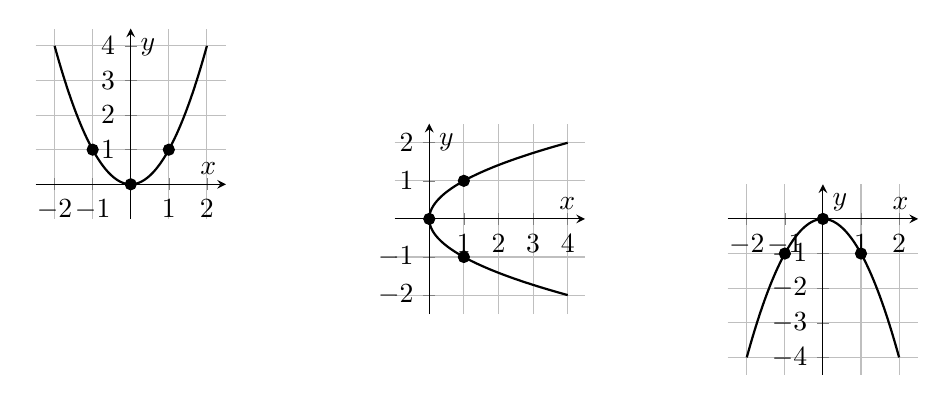
\begin{tikzpicture}
\begin{axis}[width=4cm,height=4cm,axis lines=middle,xmin=-2.5,xmax=2.5,ymin=-1,ymax=4.5,xtick={-2,-1,0,1,2},ytick={0,1,2,3,4},xlabel={$x$},ylabel={$y$},grid=both]
\addplot[domain=-2:2,samples=100,thick] {x^2};
\addplot[only marks,mark=*] coordinates {(-1,1) (0,0) (1,1)};
\end{axis}
\begin{axis}[at={(5.0cm,0)},anchor=origin,width=4cm,height=4cm,axis lines=middle,xmin=-1,ymax=2.5,xmax=4.5,ymin=-2.5,xtick={0,1,2,3,4},ytick={-2,-1,0,1,2},xlabel={$x$},ylabel={$y$},grid=both]
\addplot[domain=-2:2,samples=100,thick] ({x^2},{x});
\addplot[only marks,mark=*] coordinates {(1,-1) (0,0) (1,1)};
\end{axis}
\begin{axis}[at={(10.0cm,0)},anchor=origin,width=4cm,height=4cm,axis lines=middle,xmin=-2.5,xmax=2.5,ymin=-4.5,ymax=1,xtick={-2,-1,0,1,2},ytick={-4,-3,-2,-1,0},xlabel={$x$},ylabel={$y$},grid=both]
\addplot[domain=-2:2,samples=100,thick] {-x^2};
\addplot[only marks,mark=*] coordinates {(-1,-1) (0,0) (1,-1)};
\end{axis}
\end{tikzpicture}
\end{center}

A. Which two graphs represent the inverse of each other? Explain.

B. Look for Relationships What is the relationship between the domain and the range of the two inverse relations?

\answer{A. The 2 graphs on the left are inverses of each other. Looking at the two graphs, the left graph has points $(-1,1)$, $(0,0)$, and $(1,1)$, and the middle graph has points $(1,-1)$, $(0,0)$, and $(1,1)$. Since the $x$- and $y$-values for the two graphs are interchanged, the graphs are inverses of each other.

B. The domain of the left graph, all real numbers, is the same as the range of the middle graph. The range of the left graph, $\uncertain{y\ge 0}{source rendering could be y>0}$, is equivalent to the domain of the middle graph, $\uncertain{x\ge 0}{source rendering could be x>0}$.}
\end{model-discuss}

\begin{te-addendum}{ModelDiscuss}{LearnTogether}
Before WHOLE CLASS: Implement Tasks that Promote Reasoning and Problem Solving.

Q: How are the graphs similar? How are they different?
\answer{All three graphs are parabolas with a vertex at $(0,0)$, but they open in different directions.}

During SMALL GROUP: Support Productive Struggle in Learning Mathematics.

Q: How do the graphs of the inverse functions $y=2x+4$ and $y=\frac{1}{2}x-2$ help you understand this problem?
\answer{The graphs of these two inverse linear functions are reflections of each other across the line $y=x$, not across the $x$-axis. The same idea can be applied to determining which parabolas are inverses of each other.}

Q: How could you represent the domain and the range of each graph in order to compare them?
\answer{Write each domain and range as an inequality.}

For Early Finishers

Q: Study the graph that is not an inverse of the others. Describe the graph in terms of one of the other two. Then, describe the graph of the inverse of the function whose inverse is not shown.
\answer{The third graph is a reflection of the first graph across the $x$-axis. The graph of the inverse is a parabola with the vertex at $(0,0)$ that opens to the left.}

After WHOLE CLASS: Facilitate Meaningful Mathematical Discourse.

Q: What did you notice about the graphs that were inverses?
\answer{The graphs that are inverses of each other are reflections across the line $y=x$.}
\end{te-addendum}

\begin{te-addendum}{ModelDiscuss}{HabitsOfMind}
Communicate Precisely How are the points on graphs of functions that are inverses of each other related?
\answer{The $x$-values of a function are the $y$-values of its inverse, and the $y$-values of a function are the $x$-values of its inverse.}
\end{te-addendum}

\begin{te-addendum}{Lesson}{GeneralizeETP}
Introduce the lesson by helping students recall the inverse relationship between logarithmic and exponential functions. Explain that understanding this relationship will help them to identify and use the key features of the graphs of logarithmic functions.
\end{te-addendum}

\begin{concept-box}
LOOK FOR RELATIONSHIPS For each key feature of the logarithmic function, state the corresponding key feature of the exponential function.
\end{concept-box}

\begin{example}{1}
Identify Key Features of Logarithmic Functions

Graph $g(x)=\log_2 x$. What are the domain, range, $x$-intercept, and asymptote? What is the end behavior of the graph?

Logarithmic functions are inverses of exponential functions. Create tables of values for $f(x)=2^x$ and $g(x)=\log_2 x$.

\begin{center}
\begin{tabular}{c|ccccc}
\toprule
$f(x)$ & $-2$ & $-1$ & $0$ & $1$ & $2$ \\
\midrule
$y$ & $\frac14$ & $\frac12$ & $1$ & $2$ & $4$ \\
\bottomrule
\end{tabular}
\qquad
\begin{tabular}{c|ccccc}
\toprule
$g(x)$ & $\frac14$ & $\frac12$ & $1$ & $2$ & $4$ \\
\midrule
$y$ & $-2$ & $-1$ & $0$ & $1$ & $2$ \\
\bottomrule
\end{tabular}
\end{center}

Graph the functions and note the key features of $g(x)$.

\begin{center}
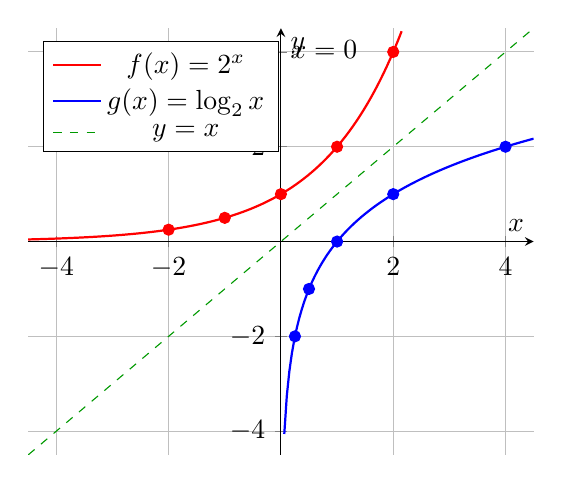
\begin{tikzpicture}
\begin{axis}[width=8cm,height=7cm,axis lines=middle,xmin=-4.5,xmax=4.5,ymin=-4.5,ymax=4.5,xtick={-4,-2,0,2,4},ytick={-4,-2,0,2,4},xlabel={$x$},ylabel={$y$},grid=both,legend style={at={(0.03,0.97)},anchor=north west}]
\addplot[red,thick,domain=-4.5:2.15,samples=100] {2^x};
\addlegendentry{$f(x)=2^x$}
\addplot[blue,thick,domain=0.06:4.5,samples=100] {ln(x)/ln(2)};
\addlegendentry{$g(x)=\log_2 x$}
\addplot[green!60!black,dashed,domain=-4.5:4.5] {x};
\addlegendentry{$y=x$}
\addplot[red,only marks,mark=*] coordinates {(-2,0.25) (-1,0.5) (0,1) (1,2) (2,4)};
\addplot[blue,only marks,mark=*] coordinates {(0.25,-2) (0.5,-1) (1,0) (2,1) (4,2)};
\draw[dashed] (axis cs:0,-4.5)--(axis cs:0,4.5) node[pos=0.95,right] {$x=0$};
\end{axis}
\end{tikzpicture}
\end{center}

The functions $f$ and $g$ are inverse functions. The graphs are reflections of each other across the line $y=x$.

Notice the ordered pairs reinforce that the functions are inverses.

The logarithmic function accepts only positive input values.

The graph of the logarithmic function approaches $x=0$ but does not touch it.

Domain: $\{x\mid x>0\}$.

Range: all real numbers.

$x$-intercept: $1$.

Asymptote: $y$-axis.

End behavior: As $x\to 0$, $y\to -\infty$. As $x\to \infty$, $y\to \infty$.

\answer{Domain: $\{x\mid x>0\}$; range: all real numbers; $x$-intercept: $1$; asymptote: $y$-axis; end behavior: As $x\to0$, $y\to -\infty$. As $x\to\infty$, $y\to\infty$.}
\end{example}

\begin{te-addendum}{1}{PurposefulQuestions}
Use and Connect Mathematical Representations

Q: When graphing $y=\log_2 x$, why is it helpful to start by graphing $y=2^x$?
\answer{The inverse relationship between exponential and logarithmic functions can be used to graph a logarithmic function.}
\end{te-addendum}

\begin{tryit}{1}
Graph each function and identify the domain and range. List any intercepts or asymptotes. Describe the end behavior.

A. $y=\ln x$

B. $y=\log_{\frac12}x$

\answer{A. Domain: $\{x\mid x>0\}$; range: all real numbers; $x$-intercept: $1$; asymptote: $y$-axis; end behavior: As $x\to0$, $y\to -\infty$. As $x\to\infty$, $y\to\infty$.

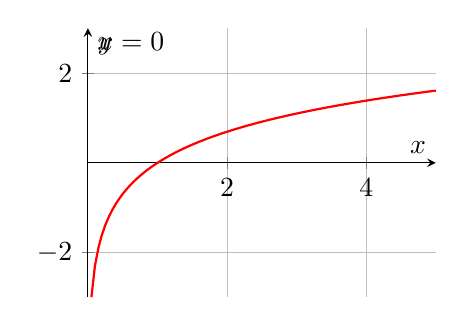
\begin{tikzpicture}
\begin{axis}[width=6cm,height=5cm,axis lines=middle,xmin=0,xmax=5,ymin=-3,ymax=3,xtick={0,2,4},ytick={-2,0,2},xlabel={$x$},ylabel={$y$},grid=both]
\addplot[red,thick,domain=0.05:5,samples=100] {ln(x)};
\draw[dashed] (axis cs:0,-3)--(axis cs:0,3) node[pos=0.95,right] {$x=0$};
\end{axis}
\end{tikzpicture}

B. Domain: $\{x\mid x>0\}$; range: all real numbers; $x$-intercept: $1$; asymptote: $y$-axis; end behavior: As $x\to0$, $y\to\infty$. As $x\to\infty$, $y\to -\infty$.

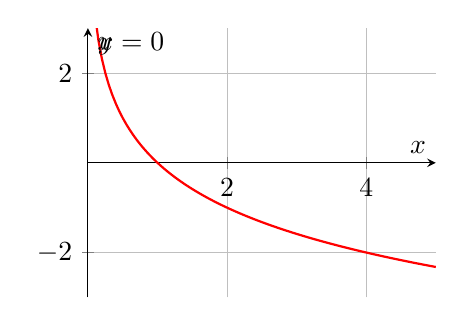
\begin{tikzpicture}
\begin{axis}[width=6cm,height=5cm,axis lines=middle,xmin=0,xmax=5,ymin=-3,ymax=3,xtick={0,2,4},ytick={-2,0,2},xlabel={$x$},ylabel={$y$},grid=both]
\addplot[red,thick,domain=0.05:5,samples=100] {ln(x)/ln(0.5)};
\draw[dashed] (axis cs:0,-3)--(axis cs:0,3) node[pos=0.95,right] {$x=0$};
\end{axis}
\end{tikzpicture}}
\end{tryit}

\begin{concept-box}
REASON Consider the transformation of a parent function translated by $(h,k)$ so that $g(x)=f(x+h)+k$. With exponential functions, the value of $k$ dictates the shift of the horizontal asymptote. With logarithmic functions, the value of $h$ determines the shift of the asymptote.
\end{concept-box}

\begin{example}{2}
Graph Transformations of Logarithmic Functions

Graph the function $g(x)=\log_2(x+3)$. How do the asymptote and $x$-intercept of the given function compare to those of the parent function $f(x)=\log_2 x$?

\[
f(x)=\log_2 x
\]
\[
g(x)=\log_2(x+3)=f(x-(-3))
\]

Since $g(x)=f(x+3)$, then $g$ is the logarithmic function translated 3 units to the left.

The vertical asymptote and the $x$-intercept each shift 3 units to the left.

\begin{center}
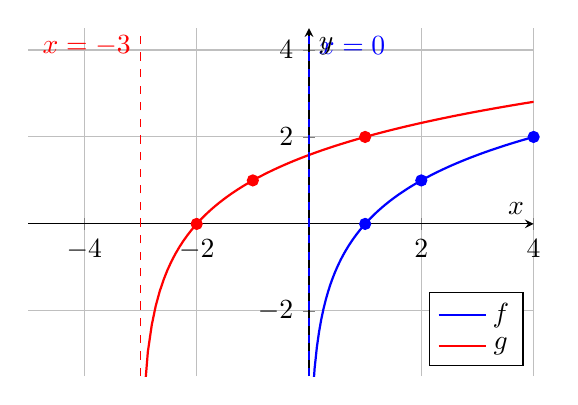
\begin{tikzpicture}
\begin{axis}[width=8cm,height=6cm,axis lines=middle,xmin=-5,xmax=4,ymin=-3.5,ymax=4.5,xtick={-4,-2,0,2,4},ytick={-2,0,2,4},xlabel={$x$},ylabel={$y$},grid=both,legend style={at={(0.98,0.03)},anchor=south east}]
\addplot[blue,thick,domain=0.06:4,samples=100] {ln(x)/ln(2)};
\addlegendentry{$f$}
\addplot[red,thick,domain=-2.94:4,samples=100] {ln(x+3)/ln(2)};
\addlegendentry{$g$}
\draw[dashed,blue] (axis cs:0,-3.5)--(axis cs:0,4.5) node[pos=0.95,right] {$x=0$};
\draw[dashed,red] (axis cs:-3,-3.5)--(axis cs:-3,4.5) node[pos=0.95,left] {$x=-3$};
\addplot[blue,only marks,mark=*] coordinates {(1,0) (2,1) (4,2)};
\addplot[red,only marks,mark=*] coordinates {(-2,0) (-1,1) (1,2)};
\end{axis}
\end{tikzpicture}
\end{center}

\answer{The vertical asymptote and the $x$-intercept each shift 3 units to the left.}
\end{example}

\begin{te-addendum}{2}{PurposefulQuestions}
Use and Connect Mathematical Representations

Q: How is graphing transformations of logarithmic functions the same as graphing transformations of exponential functions? How is it different?
\answer{Same: $h=-3$ implies a shift to the left; different: $h$ causes the shift in the asymptote of a logarithmic function, whereas $k$ causes the shift of the asymptote in an exponential function.}
\end{te-addendum}

\begin{te-addendum}{1--2}{HabitsOfMind}
Use Structure Does the graph of either $y=\ln x+4$ or $y=\ln(x+4)$ have an intercept that is different from the intercept of $y=\ln x$? Explain.
\answer{The $x$-intercept of $y=\ln x+4$ is different from the $x$-intercept of $y=\ln x$, and $y=\ln x+4$ does not have a $y$-intercept. The $x$-intercept of $y=\ln(x+4)$ is different from the $x$-intercept of $y=\ln x$ and $y=\ln(x+4)$ has a $y$-intercept.}
\end{te-addendum}

\begin{te-addendum}{2}{RtISupport}
USE WITH EXAMPLE 2 Some students may have difficulty comparing the graph of the function to the parent function. Have students practice finding the $x$-intercept or the asymptote of each function.

Q: Find the $x$-intercept of $g(x)=\log(x-5)$.
\answer{6}

Q: Find the asymptote of $h(x)=\log(x+3)$.
\answer{$x=-3$}

Q: How does the graph of $h(x)=\log(x+3)$ compare to the parent function $f(x)=\log x$?
\answer{The graph of $h$ is shifted 3 units to the left of the graph of $f$.}
\end{te-addendum}

\begin{te-addendum}{2}{LearnTogether}
ADDITIONAL EXAMPLE 2

Graph the function $f(x)=-\log(x+3)-4$. How does the graph of the function compare to that of the parent function?

Compared to the graph of $y=\log x$:

The value of $h$ is $-3$, so the vertical asymptote is translated 3 units to the left.

The value of $a$ is negative, so the graph is reflected over the $x$-axis.

The value of $k$ is $-4$, so the graph is translated 4 units down.

\begin{center}
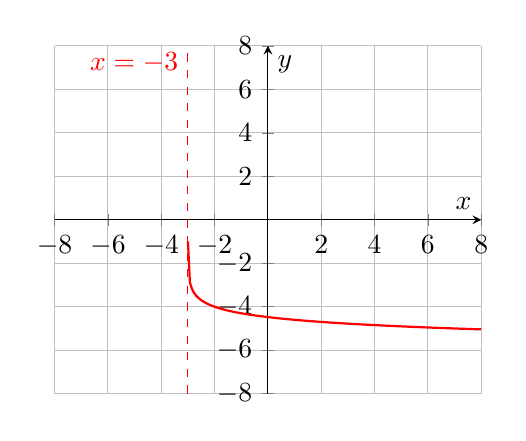
\begin{tikzpicture}
\begin{axis}[width=7cm,height=6cm,axis lines=middle,xmin=-8,xmax=8,ymin=-8,ymax=8,xtick={-8,-6,-4,-2,0,2,4,6,8},ytick={-8,-6,-4,-2,0,2,4,6,8},xlabel={$x$},ylabel={$y$},grid=both]
\addplot[red,thick,domain=-2.999:8,samples=150] {-ln(x+3)/ln(10)-4};
\draw[red,dashed] (axis cs:-3,-8)--(axis cs:-3,8) node[pos=0.95,left] {$x=-3$};
\end{axis}
\end{tikzpicture}
\end{center}

Q: How do the vertical asymptote and the $x$-intercept of $f(x)$ compare to the vertical asymptote and the $x$-intercept of $g(x)=\log(x+3)+4$?
\answer{They are the same for both functions.}
\end{te-addendum}

\begin{tryit}{2}
Describe how each graph compares to the graph of $f(x)=\ln x$.

A. $g(x)=\ln x+4$

B. $h(x)=5\ln x$

\answer{A. translated up 4 units.

B. vertical stretch of 5.}
\end{tryit}

\begin{concept-box}
LOOK FOR RELATIONSHIPS $f(x)$ is a translation of the parent function $y=10^x$ one unit left. $f^{-1}(x)$ is a translation of the parent function $y=\log x$ one unit down. Graphical translations of a function and its inverse are directly related. Explain.
\end{concept-box}

\begin{example}{3}
Inverses of Exponential and Logarithmic Functions

What is the equation of the inverse of the functions?

A. $f(x)=10^{x+1}$

\[
y=10^{x+1}
\]
\[
x=10^{y+1}
\]
\[
y+1=\log x
\]
\[
y=\log x-1
\]

The equation of the inverse of $f(x)=10^{x+1}$ is $f^{-1}(x)=\log x-1$.

Verify by function composition.

\[
f(f^{-1}(x))=10^{(\log x-1)+1}=10^{\log x}=x
\]
\[
f^{-1}(f(x))=\log 10^{x+1}-1=x+1-1=x
\]

\begin{center}
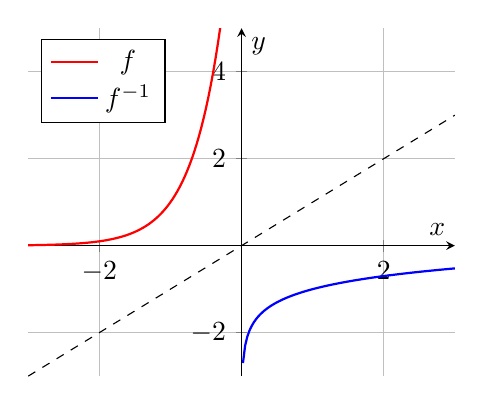
\begin{tikzpicture}
\begin{axis}[width=7cm,height=6cm,axis lines=middle,xmin=-3,xmax=3,ymin=-3,xmax=3,ymax=5,xtick={-2,0,2},ytick={-2,0,2,4},xlabel={$x$},ylabel={$y$},grid=both,legend style={at={(0.03,0.97)},anchor=north west}]
\addplot[red,thick,domain=-3:0.3,samples=100] {10^(x+1)};
\addlegendentry{$f$}
\addplot[blue,thick,domain=0.02:3,samples=100] {ln(x)/ln(10)-1};
\addlegendentry{$f^{-1}$}
\addplot[dashed,domain=-3:3] {x};
\end{axis}
\end{tikzpicture}
\end{center}

B. $g(x)=\log_7(x+5)$

\[
y=\log_7(x+5)
\]
\[
x=\log_7(y+5)
\]
\[
y+5=7^x
\]
\[
y=7^x-5
\]

The equation of the inverse of $g(x)=\log_7(x+5)$ is $g^{-1}(x)=7^x-5$.

Verify by function composition.

\[
g(g^{-1}(x))=\log_7(7^x-5+5)=\log_7 7^x=x
\]
\[
g^{-1}(g(x))=7^{\log_7(x+5)}-5=x+5-5=x
\]

\begin{center}
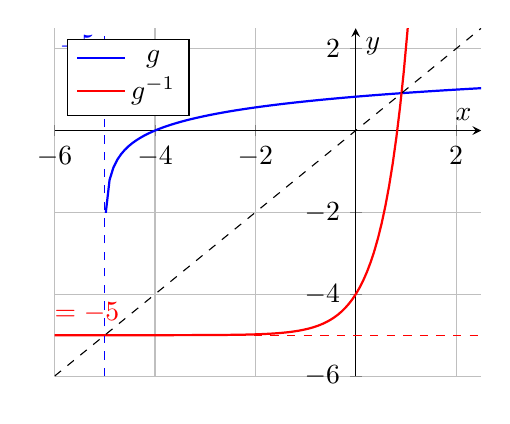
\begin{tikzpicture}
\begin{axis}[width=7cm,height=6cm,axis lines=middle,xmin=-6,xmax=2.5,ymin=-6,ymax=2.5,xtick={-6,-4,-2,0,2},ytick={-6,-4,-2,0,2},xlabel={$x$},ylabel={$y$},grid=both,legend style={at={(0.03,0.97)},anchor=north west}]
\addplot[blue,thick,domain=-4.98:2.5,samples=100] {ln(x+5)/ln(7)};
\addlegendentry{$g$}
\addplot[red,thick,domain=-6:1.25,samples=100] {7^x-5};
\addlegendentry{$g^{-1}$}
\addplot[dashed,domain=-6:2.5] {x};
\draw[blue,dashed] (axis cs:-5,-6)--(axis cs:-5,2.5) node[pos=0.95,left] {$x=-5$};
\draw[red,dashed] (axis cs:-6,-5)--(axis cs:2.5,-5) node[pos=0.05,above] {$y=-5$};
\end{axis}
\end{tikzpicture}
\end{center}

Rewrite the function as $y=$, interchange $x$ and $y$, and solve for $y$.

\answer{A. $f^{-1}(x)=\log x-1$.

B. $g^{-1}(x)=7^x-5$.}
\end{example}

\begin{te-addendum}{3}{PurposefulQuestions}
Support Productive Struggle in Learning Mathematics

Q: Why does a horizontal shift in an exponential equation become a vertical shift in its inverse?
\answer{With inverse functions, the $x$ and $y$ values are interchanged. So a transformation that affected the $x$ values of the original function would affect the $y$ values of its inverse.}
\end{te-addendum}

\begin{te-addendum}{3}{RtIExtend}
USE WITH EXAMPLE 3 Have students explore finding the inverse of functions with two translations.

Have students find the inverse of each function.

1. $f(x)=2^{x+3}-3$
\answer{$f^{-1}(x)=\log_2(x+3)-3$}

2. $g(x)=\log_4(x-4)-1$
\answer{$g^{-1}(x)=4^{x+1}+4$}

3. $h(x)=-\log(x+1)+6$
\answer{$h^{-1}(x)=10^{6-x}-1$}

Q: How are the graphs of these functions and their inverses related?
\answer{The graphs of the inverses are reflections of the original function across the line $y=x$.}
\end{te-addendum}

\begin{te-addendum}{3}{LearnTogether}
ADDITIONAL EXAMPLE 3

Find the inverse of the function.

\[
f(x)=11(4)^{x-6}+9
\]

\[
y=11(4)^{x-6}+9
\]
\[
x=11(4)^{y-6}+9
\]
\[
x-9=11(4)^{y-6}
\]
\[
\frac{x-9}{11}=(4)^{y-6}
\]
\[
y-6=\log_4\left(\frac{x-9}{11}\right)
\]
\[
y=\log_4\left(\frac{x-9}{11}\right)+6
\]

The inverse of $f(x)$ is $f^{-1}(x)=\log_4\left(\frac{x-9}{11}\right)+6$.

Q: How does knowing that logarithm functions and exponential functions are inverses help you solve this problem?
\answer{Knowing that they are inverses helps you see an overall direction for solving if you get stuck after you exchange the $x$ and $y$ variables.}
\end{te-addendum}

\begin{te-addendum}{3}{ELLAddendum}
SPEAKING BEGINNING In small groups, have students discuss the meanings of \emph{inter-} and \emph{change}, and how they relate to the meaning of \emph{interchange}.

Q: Where do you hear the word \emph{interchange} used?
\answer{Sample: when merging from one highway to another}

Q: What does the word \emph{interchange} mean?
\answer{a mutual, or reciprocal, exchange}

LISTENING DEVELOPING Have students listen to the definition of \emph{inverse} and answer the question. The definition of \emph{inverse} is the opposite or reverse of something.

Q: What does inverse mean in math?
\answer{opposite operations such as addition and subtraction; exchanging $x$ and $y$ in functions}

WRITING EXPANDING Have one student hold a card with X on it and another student hold a card with Y on it. Ask them to come to the front of the room and exchange the cards.

Q: What word from the example was just demonstrated?
\answer{interchange}

Q: Write definitions for \emph{interchange} and \emph{inverse} in your own words. Explain how the two words are related.
\answer{Check students' work.}
\end{te-addendum}

\begin{tryit}{3}
Find the inverse of each function. Then verify they are inverses by composition.

A. $f(x)=3^{x+2}$

B. $g(x)=\log_7 x-2$

\answer{A. $f^{-1}(x)=\log_3 x-2$.

B. $g^{-1}(x)=7^{x+2}$.}
\end{tryit}

\begin{concept-box}
STUDY TIP The original equation is a logarithmic function, while the rearranged equation is an exponential function. The exponential function is the inverse of the logarithmic function.
\end{concept-box}

\begin{example}{4}
Use a Logarithmic Function as a Model

A logarithmic function can approximate the altitude of a plane over time.

\placeholder{illustration}{Airplane taking off with model label $A=9{,}200\ln t+10{,}000$; label "$t$ is time in minutes after take off"; label "$A$ is altitude in feet."}

A. What is the altitude of the plane 10 minutes after takeoff?

Substitute 10 for $t$ in the equation of the function.

\[
A=9{,}200\ln 10+10{,}000
\]
\[
\approx 9{,}200(2.303)+10{,}000
\]
\[
\approx 21{,}188+10{,}000
\]
\[
\approx 31{,}188
\]

After 10 minutes, the plane's altitude is about $31{,}188$ feet.

B. How long after takeoff will the plane reach an altitude of $35{,}000$ feet?

Rearrange the equation to isolate the variable $t$.

\[
A=9{,}200\ln t+10{,}000
\]
\[
A-10{,}000=9{,}200\ln t
\]
\[
\frac{A-10{,}000}{9{,}200}=\ln t
\]
\[
t=e^{\left(\frac{A-10{,}000}{9{,}200}\right)}
\]

In the rearranged equation, time is a function of altitude, so use substitution to find time.

\[
t=e^{\left(\frac{35{,}000-10{,}000}{9{,}200}\right)}
\]
\[
\approx 15.14
\]

The plane will reach an altitude of $35{,}000$ feet after about $15.14$ minutes.

C. Evaluate the model against the altitude of the plane.

On the domain interval $(0,0.337)$ the logarithmic function is negative. The altitude of the plane is not correct during this interval. Also, the plane starts at the origin, which is on the asymptote of the model.

\answer{A. About $31{,}188$ feet. B. About $15.14$ minutes. C. On the domain interval $(0,0.337)$ the logarithmic function is negative. The altitude of the plane is not correct during this interval. Also, the plane starts at the origin, which is on the asymptote of the model.}
\end{example}

\begin{te-addendum}{4}{PurposefulQuestions}
Pose Purposeful Questions

Q: Why does it make sense that the function is not defined for negative values of $t$?
\answer{Negative values of $t$ correspond to times before takeoff, which is when the plane is constantly on the ground.}
\end{te-addendum}

\begin{te-addendum}{3--4}{HabitsOfMind}
Reason Does it make sense that the plane is at $31{,}528$ feet after 10 minutes but only $35{,}000$ feet after $15.14$ minutes?
\answer{Yes, because the rate of increase of a logarithmic function decreases as $t$ increases.}
\end{te-addendum}

\begin{tryit}{4}
Commercial airplanes usually fly no higher than $38{,}000$ ft. How long will it take the plane to reach this altitude? How does a maximum cruising height compare with the model?

\answer{About 21 minutes; The model is not accurate past 21 minutes since the logarithmic function continues to increase above the cruising altitude.}
\end{tryit}

\begin{concept-summary}
CONCEPT SUMMARY Logarithmic Functions

\begin{center}
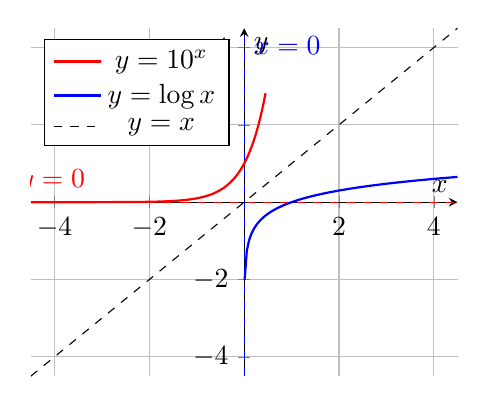
\begin{tikzpicture}
\begin{axis}[width=7cm,height=6cm,axis lines=middle,xmin=-4.5,xmax=4.5,ymin=-4.5,ymax=4.5,xtick={-4,-2,0,2,4},ytick={-4,-2,0,2,4},xlabel={$x$},ylabel={$y$},grid=both,legend style={at={(0.03,0.97)},anchor=north west}]
\addplot[red,thick,domain=-4.5:0.45,samples=100] {10^x};
\addlegendentry{$y=10^x$}
\addplot[blue,thick,domain=0.01:4.5,samples=100] {ln(x)/ln(10)};
\addlegendentry{$y=\log x$}
\addplot[dashed,domain=-4.5:4.5] {x};
\addlegendentry{$y=x$}
\draw[blue,dashed] (axis cs:0,-4.5)--(axis cs:0,4.5) node[pos=0.95,right] {$x=0$};
\draw[red,dashed] (axis cs:-4.5,0)--(axis cs:4.5,0) node[pos=0.05,above] {$y=0$};
\end{axis}
\end{tikzpicture}
\end{center}

The functions are inverses so their graphs are reflections of each other across the line with equation $y=x$.

\begin{center}
\begin{tabular}{lll}
\toprule
 & $y=\log x$ & $y=10^x$ \\
\midrule
Equations & $y=\log x$ & $y=10^x$ \\
Key Features & Domain: $\{x\mid x>0\}$ & Domain: all real numbers \\
 & Range: all real numbers & Range: $\{y\mid y>0\}$ \\
 & $x$-intercept: $1$ & $y$-intercept: $1$ \\
 & Asymptote: $y$-axis & Asymptote: $x$-axis \\
End Behavior & As $x\to0$, $y\to-\infty$ & As $x\to-\infty$, $y\to0$ \\
 & As $x\to\infty$, $y\to\infty$ & As $x\to\infty$, $y\to\infty$ \\
\bottomrule
\end{tabular}
\end{center}
\end{concept-summary}

\begin{te-addendum}{ConceptSummary}{PurposefulQuestions}
Q: How are the domain and the range of $y=\log x$ related to the domain and the range of $y=10^x$?
\answer{The domain of $y=\log x$ is the same as the range of $y=10^x$ and the range of $y=\log x$ is the same as the domain of $y=10^x$.}

Q: How are the $x$-intercept and the asymptote of $y=\log x$ affected if the graph is translated 3 units to the right?
\answer{The $x$-intercept and asymptote are also translated 3 units to the right. The $x$-intercept is 4 and the asymptote is $x=3$.}
\end{te-addendum}

\begin{te-addendum}{5}{CommonError}
Exercise 5 Students may ignore the $-1$ before adding $1\frac12$, writing the equation as $g(x)=\ln x+1\frac12$, instead of $g(x)=\ln x+\frac12$. Explain that the graph of $f(x)=\ln x-1$ is the graph of $h(x)=\ln x$ shifted down 1 unit, so shifting this function up by $1\frac12$ units is the same as shifting $h(x)$ up $\frac12$ unit.
\end{te-addendum}

\begin{practice}{1}{\uncertain{not listed}{Item Analysis table begins at item 7}}
Do You UNDERSTAND? ESSENTIAL QUESTION How is the relationship between logarithmic and exponential functions revealed in the key features of their graphs?
\answer{The domain of the logarithmic function is the same as the range of the exponential function, and the range of the logarithmic function is the same as the domain of the exponential function. The logarithmic function has an $x$-intercept of 1, while the exponential function has a $y$-intercept of 1.}
\end{practice}

\begin{practice}{2}{\uncertain{not listed}{Item Analysis table begins at item 7}}
Error Analysis Raynard claims the domain of the function $y=\log_3 x$ is all real numbers. Explain the error Raynard made.
\answer{This is the range of the function. The domain is $\{x\mid x>0\}$.}
\end{practice}

\begin{practice}{3}{\uncertain{not listed}{Item Analysis table begins at item 7}}
Communicate Precisely How are the graphs of $f(x)=\log_5 x$ and $g(x)=-\log_5 x$ related?
\answer{The graph of $g(x)$ is the reflection of the graph of $f(x)$ across the $x$-axis.}
\end{practice}

\begin{practice}{4}{\uncertain{not listed}{Item Analysis table begins at item 7}}
Use Structure Explain the necessary steps to find the inverse of $h(x)=\log_6(x+4)$.
\answer{Rewrite the problem using $x$ and $y$, then exchange the places of the $x$ and $y$. Next solve for the $y$. In this step use the relationship between exponential and logarithmic functions. Finally, rewrite in inverse function notation. $h^{-1}(x)=6^x-4$.}
\end{practice}

\begin{practice}{5}{\uncertain{not listed}{Item Analysis table begins at item 7}}
Graph the function $y=\log_4 x$ and identify the domain and range. List any intercepts or asymptotes. Describe the end behavior.
\answer{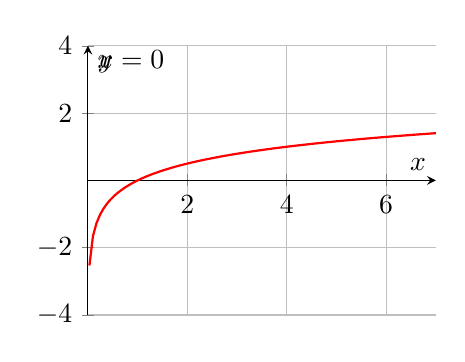
\begin{tikzpicture}
\begin{axis}[width=6cm,height=5cm,axis lines=middle,xmin=0,xmax=7,ymin=-4,ymax=4,xtick={0,2,4,6},ytick={-4,-2,0,2,4},xlabel={$x$},ylabel={$y$},grid=both]
\addplot[red,thick,domain=0.03:7,samples=100] {ln(x)/ln(4)};
\draw[dashed] (axis cs:0,-4)--(axis cs:0,4) node[pos=0.95,right] {$x=0$};
\end{axis}
\end{tikzpicture}

Domain: $\{x\mid x>0\}$; range: all real numbers; $x$-intercept: 1; asymptote: $y$-axis; end behavior: As $x\to0$, $y\to-\infty$. As $x\to\infty$, $y\to\infty$.}
\end{practice}

\begin{practice}{6}{\uncertain{not listed}{Item Analysis table begins at item 7}}
Write the equation for the function $g(x)$, which can be described as a vertical shift $1\frac12$ units up from the function $f(x)=\ln x-1$.
\answer{$g(x)=\ln x+\frac12$}
\end{practice}

\begin{practice}{7}{2}
The function $y=5\ln(x+1)$ gives $y$, the number of downloads, in hundreds, $x$ minutes after the release of a song. Find the equation of the inverse and interpret its meaning.

\placeholder{illustration}{Download bar labeled "Downloading...", green bar labeled "y downloads", blue bar labeled "x minutes".}
\answer{$x=e^{\frac{y}{5}}-1$; This function gives $x$, the number of minutes after the release of a song, in terms of the number of downloads in hundreds, $y$.}
\end{practice}

\begin{practice}{8}{2}
Sketch the functions represented by the tables. Identify which graph is the logarithmic function. Are the two functions inverses?

A.
\begin{center}
\begin{tabular}{c|ccccc}
\toprule
$x$ & $10^{-10}$ & $0.01$ & $1$ & $2$ & $10$ \\
\midrule
$g(x)$ & $-8$ & $0$ & $2$ & $2.301$ & $3$ \\
\bottomrule
\end{tabular}
\end{center}

B.
\begin{center}
\begin{tabular}{c|cccccc}
\toprule
$x$ & $-1$ & $0$ & $1$ & $2$ & $3$ & $4$ \\
\midrule
$h(x)$ & $0.001$ & $0.01$ & $0.1$ & $1$ & $10$ & $100$ \\
\bottomrule
\end{tabular}
\end{center}

\answer{$g(x)$ is the logarithmic function. Yes they are inverses.

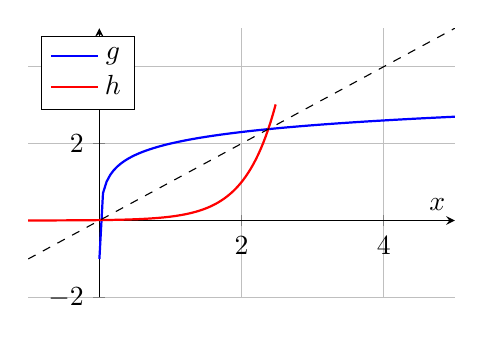
\begin{tikzpicture}
\begin{axis}[width=7cm,height=5cm,axis lines=middle,xmin=-1,xmax=5,ymin=-2,ymax=5,xtick={0,2,4},ytick={-2,0,2,4},xlabel={$x$},ylabel={$y$},grid=both,legend style={at={(0.03,0.97)},anchor=north west}]
\addplot[blue,thick,domain=0.001:5,samples=100] {ln(x)/ln(10)+2};
\addlegendentry{$g$}
\addplot[red,thick,domain=-1:2.48,samples=100] {10^(x-2)};
\addlegendentry{$h$}
\addplot[dashed,domain=-1:5] {x};
\end{axis}
\end{tikzpicture}}
\end{practice}

\begin{practice}{9}{2}
Look for Relationships Are the logarithmic and exponential functions shown inverses of each other? Explain.

\begin{center}
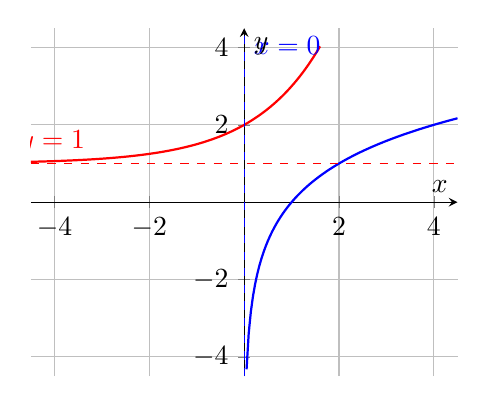
\begin{tikzpicture}
\begin{axis}[width=7cm,height=6cm,axis lines=middle,xmin=-4.5,xmax=4.5,ymin=-4.5,ymax=4.5,xtick={-4,-2,0,2,4},ytick={-4,-2,0,2,4},xlabel={$x$},ylabel={$y$},grid=both]
\addplot[red,thick,domain=-4.5:1.6,samples=100] {2^x+1};
\addplot[blue,thick,domain=0.05:4.5,samples=100] {ln(x)/ln(2)};
\draw[blue,dashed] (axis cs:0,-4.5)--(axis cs:0,4.5) node[pos=0.95,right] {$x=0$};
\draw[red,dashed] (axis cs:-4.5,1)--(axis cs:4.5,1) node[pos=0.05,above] {$y=1$};
\end{axis}
\end{tikzpicture}
\end{center}

\answer{No; The $x$-intercept of the blue function is not equal to the $y$-intercept of the red function.}
\end{practice}

\begin{practice}{10}{2}
Communicate Precisely How is the graph of the logarithmic function $g(x)=\log_2(x-7)$ related to the graph of the function $f(x)=\log_2 x$? Explain your reasoning.
\answer{$g(x)$ is shifted 7 units to the right; for each $x$, $g(x)=f(x-7)$, so the $y$-values of the functions are equal for $x$-values that are 7 units apart.}
\end{practice}

\begin{practice}{11}{2}
Error Analysis Describe and correct the error a student made in finding the inverse of the exponential function $f(x)=5^{x-6}+2$.

\begin{center}
\begin{tabular}{ll}
$y=5^{x-6}+2$ & Write in $y=f(x)$ form. \\
$x=5^{y-6}+2$ & Interchange $x$ and $y$. \\
$x-2=5^{y-6}$ & Subtract 2 from each side. \\
$y-6=\log_5x-2$ & Rewrite in logarithmic form. \\
$y=\log_5x-2+6$ & Add 6 to each side. \\
$y=\log_5x+4$ & Simplify. \\
$f^{-1}(x)=\log_5x+4$ & \\
\end{tabular}
\end{center}

\answer{When rewriting in logarithmic form, the student should have placed the expression $x-2$ in parenthesis. The correct inverse function is $f^{-1}(x)=\log_5(x-2)+6$.}
\end{practice}

\begin{practice}{12}{1}
Make Sense and Persevere The number of members $m$ who joined a new workout center $w$ weeks after opening is modeled by the equation $m=1.6^{w+2}$, where $0\le w\le10$. Find the inverse of the function and explain what the inverse tells you.
\answer{$w=\log_{1.6}m-2$; the number of weeks after opening when the number of members reaches $m$.}
\end{practice}

\begin{practice}{13}{1}
Use Structure The graph shows a transformation of the parent graph $f(x)=\log_3 x$. Write an equation for the graph.

\begin{center}
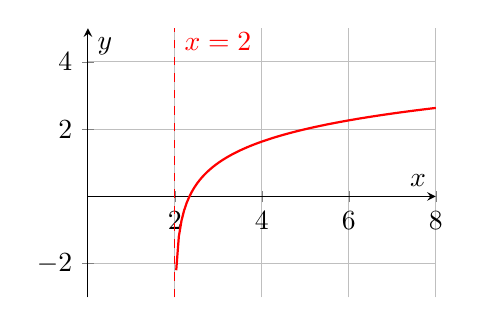
\begin{tikzpicture}
\begin{axis}[width=6cm,height=5cm,axis lines=middle,xmin=0,xmax=8,ymin=-3,ymax=5,xtick={0,2,4,6,8},ytick={-2,0,2,4},xlabel={$x$},ylabel={$y$},grid=both]
\addplot[red,thick,domain=2.03:8,samples=100] {ln(x-2)/ln(3)+1};
\draw[red,dashed] (axis cs:2,-3)--(axis cs:2,5) node[pos=0.95,right] {$x=2$};
\end{axis}
\end{tikzpicture}
\end{center}

\answer{$g(x)=\log_3(x-2)+1$}
\end{practice}

\begin{practice}{14}{1}
Graph each function and identify the domain and range. List any intercepts or asymptotes. Describe the end behavior. $y=\log_5 x$.
\answer{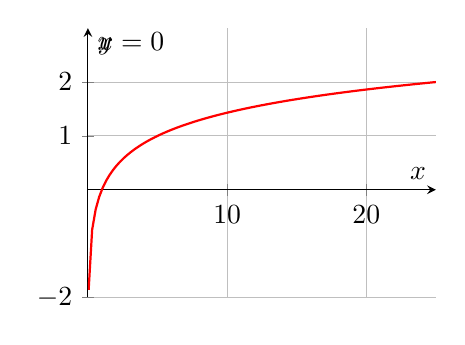
\begin{tikzpicture}
\begin{axis}[width=6cm,height=5cm,axis lines=middle,xmin=0,xmax=25,ymin=-2,ymax=3,xtick={0,10,20},ytick={-2,0,1,2},xlabel={$x$},ylabel={$y$},grid=both]
\addplot[red,thick,domain=0.05:25,samples=100] {ln(x)/ln(5)};
\draw[dashed] (axis cs:0,-2)--(axis cs:0,3) node[pos=0.95,right] {$x=0$};
\end{axis}
\end{tikzpicture}

Domain: $\{x\mid x>0\}$; range: all real numbers; intercept: $x$-intercept 1; asymptote: $y$-axis; end behavior: As $x\to0$, $y\to-\infty$. As $x\to\infty$, $y\to\infty$.}
\end{practice}

\begin{practice}{15}{1}
Graph each function and identify the domain and range. List any intercepts or asymptotes. Describe the end behavior. $y=\log_8 x$.
\answer{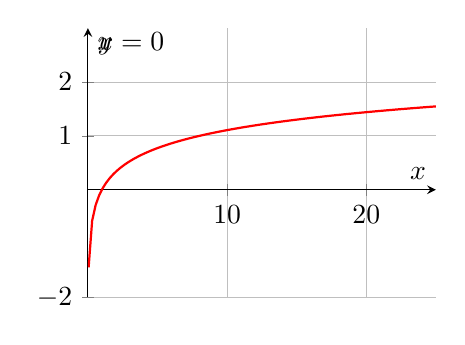
\begin{tikzpicture}
\begin{axis}[width=6cm,height=5cm,axis lines=middle,xmin=0,xmax=25,ymin=-2,ymax=3,xtick={0,10,20},ytick={-2,0,1,2},xlabel={$x$},ylabel={$y$},grid=both]
\addplot[red,thick,domain=0.05:25,samples=100] {ln(x)/ln(8)};
\draw[dashed] (axis cs:0,-2)--(axis cs:0,3) node[pos=0.95,right] {$x=0$};
\end{axis}
\end{tikzpicture}

Domain: $\{x\mid x>0\}$; range: all real numbers; $x$-intercept: 1; asymptote: $y$-axis; end behavior: As $x\to0$, $y\to-\infty$. As $x\to\infty$, $y\to\infty$.}
\end{practice}

\begin{practice}{16}{2}
Graph each function and identify the domain and range. List any intercepts or asymptotes. Describe the end behavior. $y=\log_{\frac{3}{10}}x$.
\answer{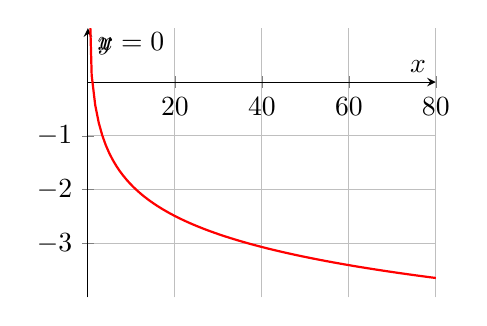
\begin{tikzpicture}
\begin{axis}[width=6cm,height=5cm,axis lines=middle,xmin=0,xmax=80,ymin=-4,ymax=1,xtick={0,20,40,60,80},ytick={-3,-2,-1,0},xlabel={$x$},ylabel={$y$},grid=both]
\addplot[red,thick,domain=0.05:80,samples=100] {ln(x)/ln(0.3)};
\draw[dashed] (axis cs:0,-4)--(axis cs:0,1) node[pos=0.95,right] {$x=0$};
\end{axis}
\end{tikzpicture}

Domain: $\{x\mid x>0\}$; range: all real numbers; intercept: $x$-intercept 1; asymptote: $y$-axis; end behavior: As $x\to0$, $y\to\infty$. As $x\to\infty$, $y\to-\infty$.}
\end{practice}

\begin{practice}{17}{2}
Graph each function and identify the domain and range. List any intercepts or asymptotes. Describe the end behavior. $y=\log_{0.1}x$.
\answer{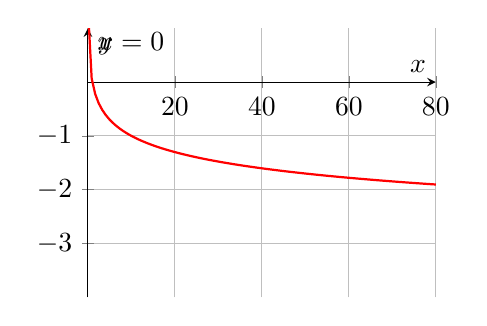
\begin{tikzpicture}
\begin{axis}[width=6cm,height=5cm,axis lines=middle,xmin=0,xmax=80,ymin=-4,ymax=1,xtick={0,20,40,60,80},ytick={-3,-2,-1,0},xlabel={$x$},ylabel={$y$},grid=both]
\addplot[red,thick,domain=0.05:80,samples=100] {ln(x)/ln(0.1)};
\draw[dashed] (axis cs:0,-4)--(axis cs:0,1) node[pos=0.95,right] {$x=0$};
\end{axis}
\end{tikzpicture}

Domain: $\{x\mid x>0\}$; range: all real numbers; intercept: $x$-intercept 1; asymptote: $y$-axis; end behavior: As $x\to0$, $y\to\infty$. As $x\to\infty$, $y\to-\infty$.}
\end{practice}

\begin{practice}{18}{2}
Describe the graph in terms of transformations of the parent function $f(x)=\log_6 x$. Compare the asymptote and $x$-intercept of the given function to the parent function. $g(x)=\frac12\log_6 x$.
\answer{Vertical shrink of $\frac12$; asymptote: $y$-axis (same as parent function); $x$-intercept 1 (same as parent function).}
\end{practice}

\begin{practice}{19}{1}
Describe the graph in terms of transformations of the parent function $f(x)=\log_6 x$. Compare the asymptote and $x$-intercept of the given function to the parent function. $g(x)=\log_6(-x)$.
\answer{Reflection over the $y$-axis; asymptote: $y$-axis (same as parent function); $x$-intercept $-1$ (different from parent function).}
\end{practice}

\begin{practice}{20}{1}
Describe how the graph of $g(x)=-\ln(x+0.5)$ is related to the graph of $f(x)=\ln x$.
\answer{Reflection of $f(x)$ shifted 0.5 units to the left.}
\end{practice}

\begin{practice}{21}{1}
Find the equation of the inverse of each function. $f(x)=5^{x-3}$.
\answer{$f^{-1}(x)=\log_5x+3$}
\end{practice}

\begin{practice}{22}{1}
Find the equation of the inverse of each function. $f(x)=\left(\frac12\right)^{x-1}$.
\answer{$f^{-1}(x)=\log_{\frac12}x+1$}
\end{practice}

\begin{practice}{23}{1}
Find the equation of the inverse of each function. $f(x)=6^{x+7}$.
\answer{$f^{-1}(x)=\log_6x-7$}
\end{practice}

\begin{practice}{24}{1}
Find the equation of the inverse of each function. $f(x)=\log_2(8x)$.
\answer{$f^{-1}(x)=\frac{2^x}{8}$}
\end{practice}

\begin{practice}{25}{2}
Find the equation of the inverse of each function. $f(x)=\ln(x+3)-1$.
\answer{$f^{-1}(x)=e^{x+1}-3$}
\end{practice}

\begin{practice}{26}{2}
Find the equation of the inverse of each function. $f(x)=4\log_2(x-3)+2$.
\answer{$f^{-1}(x)=2^{\frac{x-2}{4}}+3$}
\end{practice}

\begin{practice}{27}{2}
The altitude $y$, in feet, of a plane $t$ minutes after takeoff is approximated by the function $y=5{,}000\ln(.05t)+8{,}000$. Solve for $t$ in terms of $y$. What is a situation in which it would be easier to use your new equation rather than the original?
\answer{$t=20e^{\frac{y-8{,}000}{5{,}000}}$; Use this new equation when the altitude of the plane is known but the time since takeoff is not.}
\end{practice}

\begin{practice}{28}{3}
A company uses this function to relate sales revenue, $R$, and advertising costs, $a$. What is the equation of the inverse of the equation? Which equation would be easier to use to find a value of $a$ for a particular value of $R$?

\placeholder{illustration}{Sales revenue represented by stacks of coins labeled "Sales Revenue, R" and advertising costs represented by a web ad and phone labeled "Advertising Costs, a" with formula $R=12\log(a+1)+25$.}
\answer{The inverse of the formula is $a=10^{\frac{R-25}{12}}-1$. It would be easier to use the inverse to find $a$ when $R$ is known.}
\end{practice}

\begin{practice}{29}{2}
Model with Mathematics The equation $r=90-25\log(t+1)$ is to model a student's retention $r$ after taking a physics course where $r$ represents a student's test score (as a percent), and $t$ represents the number of months since taking the course.

A. Make a table of values for ordered pairs that represent $r=90-25\log(t+1)$, rounding to the nearest tenth. Then sketch the graph of the function on a coordinate plane through those ordered pairs. (You may use a graphing calculator to check.)

B. Find the equation of the inverse. Interpret the meaning of this function.

\answer{A. Check students' work.

\begin{tabular}{cc}
\toprule
$t$ & $r$ \\
\midrule
9 & 65 \\
99 & 40 \\
200 & 32.5 \\
300 & 28 \\
400 & 24.9 \\
\bottomrule
\end{tabular}

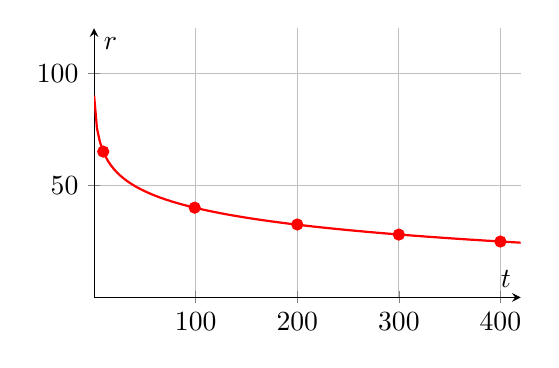
\begin{tikzpicture}
\begin{axis}[width=7cm,height=5cm,axis lines=middle,xmin=0,xmax=420,ymin=0,ymax=120,xtick={0,100,200,300,400},ytick={0,50,100},xlabel={$t$},ylabel={$r$},grid=both]
\addplot[red,thick,domain=0:420,samples=150] {90-25*ln(x+1)/ln(10)};
\addplot[red,only marks,mark=*] coordinates {(9,65) (99,40) (200,32.5) (300,28) (400,24.9)};
\end{axis}
\end{tikzpicture}

B. $t=10^{\frac{r-90}{-25}}-1$; the number of months since taking the course at which a student has a retention, $r$.}
\end{practice}

\begin{practice}{30}{1}
Higher Order Thinking As shown by the diagram, an earthquake occurs below Earth's surface at point $F$ (the focus). Point $E$, on the surface above the focus, is called the epicenter. A seismograph station at point $S$ records the waves of energy generated by the earthquake. The surface wave magnitude $M$ of the earthquake is given by this formula:

\[
M=\log\left(\frac{A}{T}\right)+1.66(\log D)+3.3
\]

In the formula, $A$ is the amplitude of the ground motion in micrometers, $T$ is the period in seconds, and $D$ is the measure of $\widehat{ES}$ in degrees.

\placeholder{illustration}{Cutaway diagram of Earth's surface with focus F below the surface, epicenter E above the focus, seismograph station S on the surface, arc ES, and waves radiating from the focus.}

A. Find surface wave magnitude of an earthquake with $A=700$ micrometers, $T=2$ and $D=100^\circ$.

B. In the formula, $20^\circ<D\le160^\circ$. By how much can the size of arc $\widehat{ES}$ affect the surface wave magnitude? Explain.

\answer{A. magnitude 9.2.

B. The size of the arc can add between 2.2 and 3.7 to the surface wave magnitude, meaning the arc size can affect the surface wave magnitude by up to 1.5.}
\end{practice}

\begin{practice}{31}{2}
The logarithmic function $g(x)=\ln x$ is transformed to $h(x)=\ln(x+2)-1$. Which of the following are true? Select all that apply.

$\square$ $g(x)$ is translated 2 units upward.

$\square$ $g(x)$ is translated 2 units to the right.

$\square$ $g(x)$ is translated 2 units to the left.

$\square$ $g(x)$ is translated 1 unit downward.

$\square$ $g(x)$ is translated 1 unit to the left.

$\square$ The vertical asymptote shifts 2 units to the left.

$\square$ The vertical asymptote shifts 2 units to the right.

\answer{$g(x)$ is translated 2 units to the left; $g(x)$ is translated 1 unit downward; The vertical asymptote shifts 2 units to the left.}
\end{practice}

\begin{practice}{32}{\uncertain{not listed}{not included in Item Analysis table}}
SAT/ACT The graph shows the exponential function $f(x)=5^x+1$. Which of the following functions represents its inverse, $f^{-1}(x)$?

\begin{center}
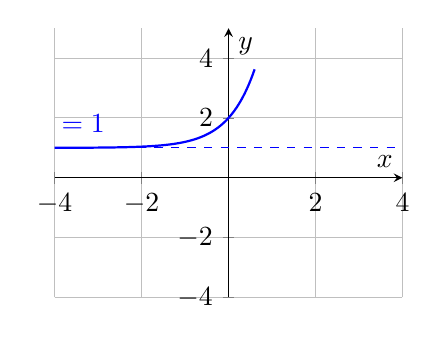
\begin{tikzpicture}
\begin{axis}[width=6cm,height=5cm,axis lines=middle,xmin=-4,xmax=4,ymin=-4,ymax=5,xtick={-4,-2,0,2,4},ytick={-4,-2,0,2,4},xlabel={$x$},ylabel={$y$},grid=both]
\addplot[blue,thick,domain=-4:0.6,samples=100] {5^x+1};
\draw[blue,dashed] (axis cs:-4,1)--(axis cs:4,1) node[pos=0.05,above] {$y=1$};
\end{axis}
\end{tikzpicture}
\end{center}

A. $f^{-1}(x)=1+\log_5x$

B. $f^{-1}(x)=\log_5x-1$

C. $f^{-1}(x)=\log_5(x-1)$

D. $f^{-1}(x)=\log_5(x+1)$

\answer{C. $f^{-1}(x)=\log_5(x-1)$}
\end{practice}

\begin{practice}{33}{\uncertain{not listed}{not included in Item Analysis table}}
Performance Task The logarithmic function $M(d)=5\log d+2$ is used to find the limiting magnitude of a telescope, where $d$ represents the diameter of the lens of the telescope (mm) that is being used for the observation.

Part A Find the limiting magnitude of a telescope having a lens diameter of 40 mm.

Part B Find the equation of the inverse of this function.

Part C Interpret why astronomers may wish to use the inverse of this function. Justify your reasoning.

Part D Using the inverse function, find the diameter of the lens that has a limiting magnitude of 13.5. Check your answer with the table function of your graphing calculator.

\answer{A. magnitude 10.

B. $d=10^{\frac{M-2}{5}}$.

C. Astronomers can use this function when the limiting magnitude of a telescope is known to find the diameter of the lens of the telescope.

D. $199.5$ mm.}
\end{practice}

\end{document}